%%%%%%%%%%%%%%%%%%%%%%%%%%%%%%%%%%%%%%%%%
% Homework Assignment Article
% LaTeX Template
% Version 1.3.1 (ECL) (08/08/17)
%
% This template has been downloaded from:
% Overleaf
%
% Original author:
% Victor Zimmermann (zimmermann@cl.uni-heidelberg.de)
%
% License:
% CC BY-SA 4.0 (https://creativecommons.org/licenses/by-sa/4.0/)
%
%%%%%%%%%%%%%%%%%%%%%%%%%%%%%%%%%%%%%%%%%

%----------------------------------------------------------------------------------------

\documentclass[a4paper]{article} % Uses article class in A4 format

\usepackage{xcolor}
\usepackage{tcolorbox}
\tcbuselibrary{breakable}
\usepackage{hyperref}
\hypersetup{
    colorlinks=true,
    linkcolor=black,
    filecolor=magenta,      
    urlcolor=cyan,
}
\usepackage{listings}
\usepackage{color}
\usepackage{subcaption}

%----------------------------------------------------------------------------------------
%	FORMATTING
%----------------------------------------------------------------------------------------

\addtolength{\hoffset}{-2.25cm}
\addtolength{\textwidth}{4.5cm}
\addtolength{\voffset}{-3.25cm}
\addtolength{\textheight}{5cm}
\setlength{\parskip}{0pt}
\setlength{\parindent}{0in}

\renewcommand{\baselinestretch}{1.5}

%----------------------------------------------------------------------------------------
%	PACKAGES AND OTHER DOCUMENT CONFIGURATIONS
%----------------------------------------------------------------------------------------

\usepackage{blindtext} % Package to generate dummy text

\usepackage{charter} % Use the Charter font
\usepackage[utf8]{inputenc} % Use UTF-8 encoding
\usepackage{microtype} % Slightly tweak font spacing for aesthetics

\usepackage[spanish]{babel} % Language hyphenation and typographical rules

\usepackage[yyyymmdd]{datetime} % Uses YEAR-MONTH-DAY format for dates
\renewcommand{\dateseparator}{-} % Sets dateseparator to '-'

\usepackage{fancyhdr} % Headers and footers
\pagestyle{fancy} % All pages have headers and footers
\fancyhead{}\renewcommand{\headrulewidth}{0pt} % Blank out the default header
\fancyfoot[L]{} % Custom footer text
\fancyfoot[C]{} % Custom footer text
\fancyfoot[R]{\thepage} % Custom footer text

\newcommand{\note}[1]{\marginpar{\scriptsize \textcolor{red}{#1}}} % Enables comments in red on margin

%----------------------------------------------------------------------------------------

\begin{document}

%----------------------------------------------------------------------------------------
%	TITLE SECTION
%----------------------------------------------------------------------------------------

\title{Prácticas VIA} % Article title
\fancyhead[C]{}
\hrule \medskip % Upper rule
\begin{minipage}{0.295\textwidth} % Left side of title section
\raggedright
VIA\\ % Your lecture or course
\footnotesize % Authors text size
\hfill\\
Juan José Morell Fernández, 24418612H% Your name, your matriculation number
\end{minipage}
\begin{minipage}{0.4\textwidth} % Center of title section
\centering 
\large % Title text size
VISION ARTIFICIAL\\ % Assignment title and number
\normalsize % Subtitle text size
Boletin de Ejercicios\\ % Assignment subtitle
\end{minipage}
\begin{minipage}{0.295\textwidth} % Right side of title section
\raggedleft
\today\\ % Date
\footnotesize % Email text size
\hfill\\
juanjose.morellf@um.es % Your email
\end{minipage}
\medskip\hrule % Lower rule
\bigskip

\tableofcontents
\newpage

%----------------------------------------------------------------------------------------
%	ARTICLE CONTENTS
%----------------------------------------------------------------------------------------

\section{CALIBRACIÓN}

\begin{tcolorbox}[breakable,notitle,boxrule=0pt,colback=lightgray,colframe=lightgray]
a) Realiza una calibración precisa de tu cámara mediante múltiples imágenes de un chessboard. 

b) Haz una calibración aproximada con un objeto de tamaño conocido y compara con el resultado anterior. 

c) Determina a qué altura hayu que poner la cámara para obtener una vista cenital completa de un campo de baloncesto. 

d) Haz una aplicación para medir el ángulo que definen dos puntos marcados con el ratón en el imagen. 

e) Opcional: determina la posición aproximada desde la que se ha tomado una foto a partir ángulos observados respecto a puntos de referencia conocidos.
\end{tcolorbox}


Para la realización de este ejercicio se ha hecho uso de los siguientes códigos ejemplo proporcionados por el profesor:

\begin{itemize}
  \item calibrate.py
  \item undist.py
  \item medidor.py
\end{itemize}

\subsection{Apartado A}
La calibración precisa de la cámara se realizará mediante el uso de un patron con forma de tablero de ajedrez. Con el objetivo de obtener el valor FOV de la imagen tomada. Todo el proceso se realiza bajo las instrucciones marcadas en la carpeta donde se localiza \textit{calibrate.py}.\\

El procedimiento es tomar una serie de fotos en las que aparezca el patrón de ajedrez, y pasarlas como entrada al código de \textit{calibrate.py}. Este devuelve tres parámetros:
\begin{itemize}
	\item Error de ajuste. (RMS)
	\item La calibración de cámara. (K)
	\item Coeficientes de distorsión radial.
\end{itemize}

\vspace{0.3cm}

Dentro de la diagonal de la matriz K se encuentra el valor \textit{f}. Con todos estos valores se puede obtener la imagen transformada sin distorsión, mediante el uso de \textit{undist.py} pero modificando los valores de \textit{K} y \textit{D}.\\

Tras la ejecucion de los programas se obtiene un valor \textit{f} de $3.06144885e+03$ y se puede calcular el valor FOV mediante la siguiente fórmula:

\begin{center}
	$tan(\frac{FOV}{2}) = \frac{\frac{W}{2}}{\textit{f}} \rightarrow \frac{FOV}{2} = \arctan(0.4899) \rightarrow FOV = 52.2$
\end{center}

Asimismo, la información de la imagen se puede obtener a partir de los metadatos de la misma. Obteniendo que la distancia focal de la cámara es de 26 (35 mm), y mediante una tabla de referencia \cite{FOV} se puede saber que el \textbf{FOV es de 54.4}.\ \

\newpage
\subsection{Apartado B}

Para la realización de este ejercicio se ha seleccionado como objeto una libreta (\textit{Figura \ref{fig:libreta}}) con un tamaño \textit{x} de 21 cm y una distancia entre la cámara y el objeto de \textit{z} = 35 cm. Mediante el programa \textit{medidor.py} se obtiene que la medida del objeto en pixeles es de u = 1904 pixeles.

\vspace{0.3cm}

\begin{figure}[htp]
	\centering
	\includegraphics[width=5cm]{imagenes/libreta.jpg}
	\caption{Imagen Apartado B}
	\label{fig:libreta}
\end{figure}

Una vez obtenidos todas las medidas se aplica la siguiente fórmula, para obtener el valor de \textit{f}:
\begin{center}
	$u = \textit{f} \frac{X}{Z} \rightarrow 1904 = \textit{f} \frac{21}{35} \rightarrow \textit{f} = 3173'3 pixels$
\end{center}

Del mismo modo, se calcula el valor de FOV (teniendo en cuenta que las dimensiones de la imagen tomada son: w = 3000 y h = 4000):

\begin{center}
	$tan(\frac{FOV}{2}) = \frac{\frac{W}{2}}{\textit{f}} \rightarrow tan(\frac{FOV}{2}) = 0.473 \rightarrow \frac{FOV}{2} = \arctan (0.473) \rightarrow FOV = 50.63$
\end{center}

De manera que, el valor FOV (horizontal) obtenido a partir de un objeto con tamaño conocido es de \textbf{50.63}, que difiere menos de un 30\% con el valor obtenido en la calibración precisa.

\subsection{Apartado C}

Este apartado es parecido al anterior, pero se busca una distancia entre la cámara y el campo (\textit{z}) para que este se vea en su totalidad.

Para esto se nombran los siguientes datos conocidos:
\begin{itemize}
	\item Focal Lenght = 26 (35mm)
	\item FOV = 52.2
	\item h = 15000 cm (dim. campo basket)
	\item w = 28000 cm (dim. campo basket)
	\item h = 4000 pixels (dim. imagen cámara)
	\item h = 3000 pixels (dim. imagen cámara)
\end{itemize}

\newpage
Por último, el cálculo sería el siguiente:

\begin{center}
	$tan(\frac{FOV}{2}) = \frac{\frac{W}{2}}{\textit{f}} \rightarrow tan(\frac{52.2}{2}) = \frac{\frac{3000}{2}}{\textit{f}} \rightarrow \textit{f} = 3061.88 pixels$
\end{center}
\begin{center}
	$u = \textit{f} \frac{X}{Z} \rightarrow 4000 = 3061.88 * \frac{15000}{z} \rightarrow z = 11.48 m$
\end{center}

El resultado obtenido es que la distancia a la que se debe colocar la cámara para captar la totalidad del campo es de \textbf{11,48 m} de altura.

\subsection{Apartado D}

Para lograr medir el ángulo entre dos puntos, tomo como esqueleto el código de \textit{medidor.py} y un artículo web \cite{Angulos} donde se explica este concepto.

\begin{figure}[htp]
	\centering
	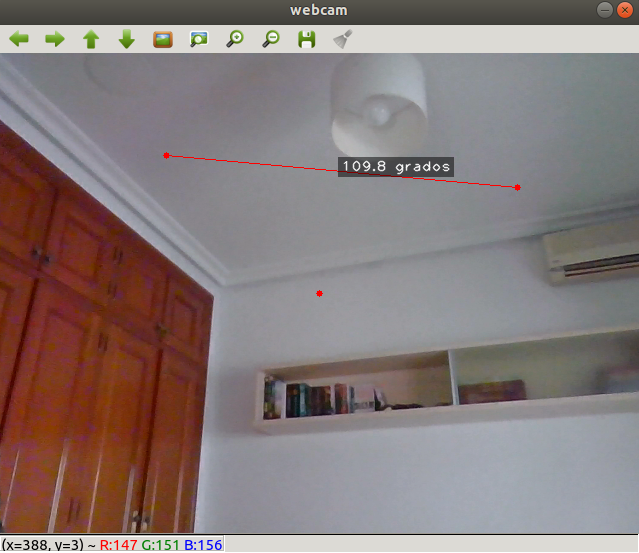
\includegraphics[width=7cm]{imagenes/angulo.png}
	\caption{Programa para medir ángulos}
	\label{fig:libreta}
\end{figure}

La idea es que mediante el punto central de la imagen, obtener dos vectores desde esta a los otros dos puntos y calcular el ángulo entre dichos vectores.\\

\begin{tcolorbox}[]
\begin{lstlisting}[language=Python]
def getAngle(a, b, c):
	a = np.array(a)
	b = np.array(b)
	c = np.array(c)
			
	ba = a - b
	bc = c - b
			
	cosine_angle = np.dot(ba, bc) / (np.linalg.norm(ba) 
	                                 * np.linalg.norm(bc))
	angle = np.arccos(cosine_angle))
	return np.degrees(angle)
\end{lstlisting}
\end{tcolorbox}

\subsection*{Manual de Usuario}

El archivo que contiene el programa de \textit{Medidor de Ángulos} tiene el nombre de \textit{medidor.py}. Y para ejecutarlo, será necesario introducir el siguiente comando en el directorio donde se encuentre dicho archivo:
\\
\begin{tcolorbox}[collower=red!75!black]
	python \textbf{medidor.py}
	\tcblower
	- -dev : Seleccionar dispositivo de entrada.
\end{tcolorbox}

\subsection{Apartado E}
...

\newpage

%------------------------------------------------

\section{ACTIVIDAD}
\bigskip

\begin{tcolorbox}[breakable,notitle,boxrule=0pt,colback=lightgray,colframe=lightgray]
Construye un detector de movimiento en una región de interés de la imagen marcada manualmente. Guarda 2 ó 3 segundos de la secuencia detectada en un archivo de vídeo. Opcional: muestra el objeto seleccionado anulando el fondo.
\end{tcolorbox}

Para la realización de este ejercicio se ha hecho uso de los siguientes códigos ejemplo proporcionados por el profesor:

\begin{itemize}
  \item roi.py
  \item video\_save.py
\end{itemize}

\subsection{Detector de Movimiento}
El dectector de movimiento se basa en la idea de tomar una instantanea en el momento que se selecciona una region y utilizarla como imagen \textit{background}, donde si se produce algún cambio sobre ella se detectaría una actividad no esperada.\\

\begin{tcolorbox}[]
\begin{lstlisting}[language=Python]
frameROI = frame[y1:y2+1, x1:x2+1]
gray = cv.cvtColor(frameROI, cv.COLOR_BGR2GRAY)
gray = cv.GaussianBlur(gray, (21,21), 0)

if background is None:
    background = gray

subtraction = cv.absdiff(background, gray)
threshold = cv.threshold(subtraction, 25, 255, cv.THRESH_BINARY) [1]
threshold = cv.dilate(threshold, None, iterations=2)
\end{lstlisting}
\end{tcolorbox}

Cuando se inicia la detección de actividad, si no lo hay, se asigna un nuevo background que estará transformado al espacio de color gris. Esto se hace para simplificar la ejecución del programa sin perder demasiada información.
\\
\\
Posteriormente, se realiza una resta, con la operación \textbf{\textit{absdiff}} de \textit{OpenCV}, entre la imagen de fondo y la imagen actual en busca de la existencia de alguna diferencia entre ambas. Si esta diferencia existe, significa que ha habido un cambio en la imagen, y por tanto una actividad inesperada. Asimismo, este cambio podría no ser tan significativo y solamente se trate de una diferencia mínima entre el color de la imagen, por cambios de luz o similar.
\\
\\
Para solucionar este problema se hace uso de la operación \textbf{\textit{threshold}} que aporta \textit{OpenCV}. Creando un filtro para ese tipo de condiciones, especificamente se indica un threshold mínimo de 25. \cite{threshold} Finalmente, se realiza la operación \textbf{\textit{dilate}} para podemos detectar de manera más facil los objetos/personas que han activado la actividad.
\\ 

\renewcommand{\baselinestretch}{1}
\begin{tcolorbox}[]
\begin{lstlisting}[language=Python]
im, outlines, hierarchy = cv.findContours(countorimg, cv.RETR_TREE, 
                                          cv.CHAIN_APPROX_SIMPLE)
for c in outlines:
    if cv.contourArea(c) < 500:
        continue

    (x,y,w,h) = cv.boundingRect(c)
    (x,y,w,h) = (x+x1,y+y1,w+x2,h+y2)
    cv.rectangle(frame, (x,y), (x+w,y+h), (0,255,0), 2)
\end{lstlisting}
\end{tcolorbox}
\renewcommand{\baselinestretch}{1.5}

Con esta porción de código se detectan los contornos que componen el ROI de la actividad detectada y se muestra por pantalla dibujando un cuadrado alrededor del objeto detectado. A continuación, se muestra una imagen con la demostracion del programa: mostrando el estado antes de la actividad y cuando se produce alguna actividad.

\begin{figure}[htp]
    \centering
    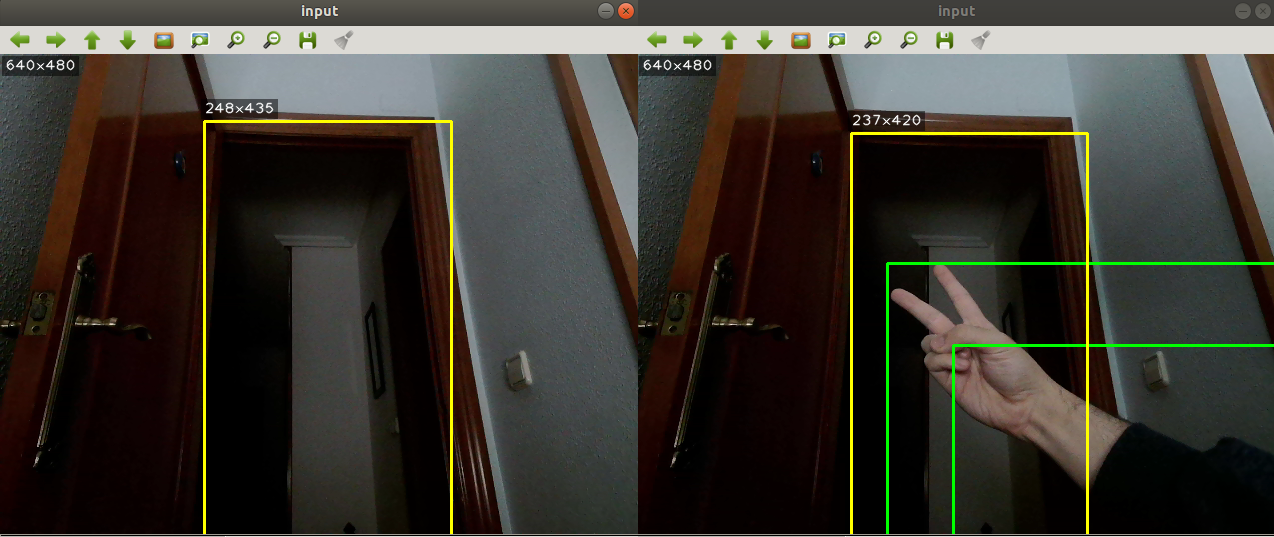
\includegraphics[width=12cm]{imagenes/ACTIVIDAD-detector.png}
    \caption{Detección de Actividad}
    \label{fig:detect}
\end{figure}


\subsection{Grabación de Video}

Para la realización de este apartado se hace una implementación del código proporcionado por el profesor, \textit{video\_save.py}. El video se va a almacenar en un archivo de salida llamado \textbf{\textit{output.mp4}} que contendrá, concatenadas, todas las actividades que se hayan reconocido durante el tiempo de ejecución del programa. En cuanto una actividad finaliza, se graban un tres segundos más.

\subsection{Anulación de Fondo}

Mediante el uso de la variable \textbf{\textit{background}} que se define en el apartado 2.1 de este ejercicio se puede realizar una anulación del fondo. Y para esto, solo es necesario realizar una resta entre este background y la imagen actual, mostrando la diferencia entre ambas. El resultado es el siguiente:

\begin{figure}[htp]
    \centering
    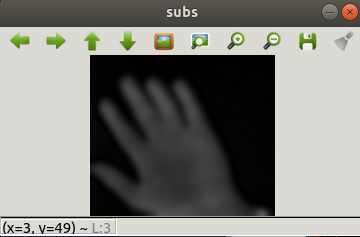
\includegraphics[width=7cm]{imagenes/anulacion.png}
    \caption{Anulación de Fondo}
    \label{fig:fondo}
\end{figure}

\subsection*{Manual de Usuario}

El archivo que contiene el programa de \textit{Actividad} tiene el nombre de \textit{act.py}. Y para ejecutarlo, será necesario introducir el siguiente comando en el directorio donde se encuentre dicho archivo:
\\
\begin{tcolorbox}[collower=red!75!black]
python \textbf{act.py}
\tcblower
- -dev : Seleccionar dispositivo de entrada.
\end{tcolorbox}

Operaciones durante la ejecución:

\begin{center}
    \begin{tabular}{ l | c }
      Tecla & Acción \\ \hline
      c & Guardar zona ROI \\
      x & Eliminar zona ROI \\
      d & Comenzar detección de actividad \\
    \end{tabular}
\end{center}

\newpage

%------------------------------------------------

\section{COLOR}
\bigskip

\begin{tcolorbox}[breakable,notitle,boxrule=0pt,colback=lightgray,colframe=lightgray]
Construye un clasificador de objetos en base a la similitud de los histogramas de color del ROI (de los 3 canales por separado). Opcional: Segmentación por reproyección.
\end{tcolorbox}

Para la realización de este ejercicio se ha hecho uso de los siguientes códigos ejemplo proporcionados por el profesor:

\begin{itemize}
  \item roi.py
  \item histogram.py
  \item histogram2.py
\end{itemize}

\subsection{Modelo de Histogramas}

Para la obtención de los histogramas que representan la imagen incluida en la región ROI se ha creado una función, llamada \textbf{\textit{calcBRGHist}}, que devuelve tres histogramas (uno por cada canal de color RGB). Para ello se sigue el siguiente procedimiento: 

\renewcommand{\baselinestretch}{1}
\begin{tcolorbox}[]
\begin{lstlisting}[language=Python]
def calcBRGHist(bgr_hist, hist_h):
    histSize = 256
    histRange = (0,256)
    accumulate = False
    hist_h = y2 - y1

    b_hist = cv.calcHist(bgr_hist, [0], None, [histSize], 
                         histRange, accumulate=accumulate)
    g_hist = cv.calcHist(bgr_hist, [1], None, [histSize], 
                         histRange, accumulate=accumulate)
    r_hist = cv.calcHist(bgr_hist, [2], None, [histSize], 
                         histRange, accumulate=accumulate)

    cv.normalize(b_hist, b_hist, alpha=0, beta=hist_h, 
                 norm_type=cv.NORM_MINMAX)
    cv.normalize(g_hist, g_hist, alpha=0, beta=hist_h, 
                 norm_type=cv.NORM_MINMAX)
    cv.normalize(r_hist, r_hist, alpha=0, beta=hist_h, 
                 norm_type=cv.NORM_MINMAX)

    return b_hist, g_hist, r_hist
\end{lstlisting}
\end{tcolorbox}
\renewcommand{\baselinestretch}{1.5}

\begin{enumerate}
    \item Inicialización de los parámetros necesarios para que solamente se hagan los histogramas de la región ROI.
    \item Función \textbf{\textit{calcHist}}: Calcula los histogramas para cada uno de los canales.
    \item Función \textbf{\textit{normalize}}: Se utiliza para poder comparar los histogramas de una manera más realista, ya que cada uno de los ROIs que se seleccionen no van a tener las mismas dimensiones.
\end{enumerate}

Toda esta función esta basada en el tutorial de la documentación oficial de OpenCV. \cite{histCalc}\\
A continuación, se almacenan los tres histogramas en un array llamado \textbf{\textit{modeloHist}}, que contendrá los histogramas de las tres regiones ROI que componen el modelo. Una vez almacenados, se puede proceder a la comparación con ROIs futuros de la imagen.

\subsection{Comparación de Histogramas}
Para la comparación entre histogramas, se hará uso de la documentación oficial de OpenCV sobre dicho tema. \cite{histComp} Y se crea una función llamada \textbf{\textit{compararHistogramas}}, que realizará todo el proceso de cálculo de los valores de relación entre el histograma del ROI actual con los del modelo.

\renewcommand{\baselinestretch}{1}
\begin{tcolorbox}[]
\begin{lstlisting}[language=Python]
def compararHistogramas(modelo, trozo, hist_h):
    # Histograma del trozo a comparar
    bgr_planes = cv.split(trozo)
    histSize = 256
    b_hist, g_hist, r_hist = calcBRGHist(bgr_planes, hist_h)

    valores = []
    # Comparar con los histogramas del modelo
    for [b_hist2, g_hist2, r_hist2] in modeloHist:
        b_comp = cv.compareHist(b_hist, b_hist2, cv.HISTCMP_CORREL)
        g_comp = cv.compareHist(g_hist, g_hist2, cv.HISTCMP_CORREL)
        r_comp = cv.compareHist(r_hist, r_hist2, cv.HISTCMP_CORREL)
                                
        valores.append(b_comp + g_comp + r_comp)
    return valores
\end{lstlisting}
\end{tcolorbox}
\renewcommand{\baselinestretch}{1.5}

El procedimiento que se sigue para realizar esta función es el siguiente:

\begin{enumerate}
    \item Se obtienen los histogramas de la región ROI actual.
    \item Se crea un array que contendrá los valores de comparación de cada uno de los histogramas de las imagenes del modelo.
    \item Función \textbf{\textit{compareHist}}: Se utiliza para comparar dos histogramas mediante una medida. En este caso, se utiliza la medida \textbf{\textit{HISTCMP\_CORREL}}, que es la correlación. Cuanto mayor sea su valor mas relación habra entre los histogramas de ambas imagenes.
\end{enumerate}

Por último, se selecciona la imagen del modelo más semejante a la región ROI actual recorriendo la salida de la función anterior y obteniendo el valor más alto.

\subsection{Segmentación por reproyección}

Para el desarrollo de esta parte se crea un nuevo programa python (\textit{segcolor.py}) semejante al programa de color pero solamente centrada en la explicación que se realiza en el notebook \textit{colorseg}.\\

La implementación realizada se basa en la clasificación probabilística, donde se intenta clasificar los pixeles de la imagen dependiendo de que a que clase pertenece, dentro de los colores almacenados en el modelo.

Para obtener estos colores del modelo, se sigue el siguiente procedimiento:
\begin{itemize}
	\item Se calcula el histograma de la region ROI seleccionada. (Dentro de los canales UY)
	\item Obtener la verosimilitud de cada pixel y se le aplica un filtro \textit{Gaussian} para que los pixeles vecinos influyan en casos donde la verosimilitud no es tan clara.
	\item Se normaliza las verosimilitudes y se obtiene la probabilidad.
	\item Se imprime el resultado en una imagen donde se presenta el color ganador en cada uno de los pixeles de la imagen.
\end{itemize}

El resultado obtenido es una segmentación de la imagen por color, mediante el uso de los histogramas.

\begin{figure}[htp]
	\centering
	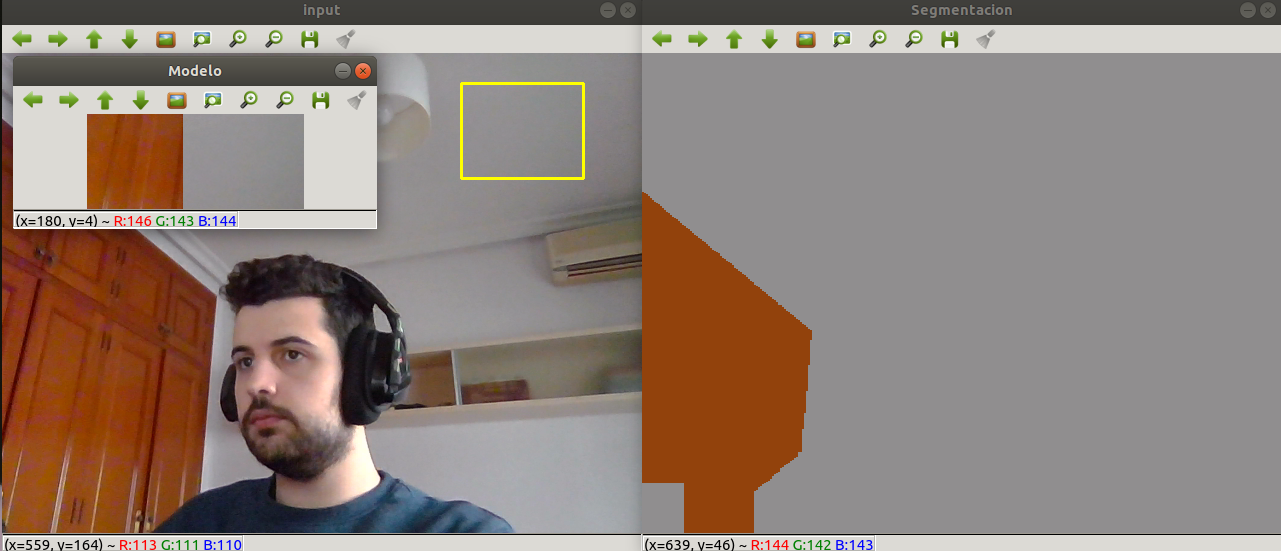
\includegraphics[width=10cm]{imagenes/seg.png}
	\caption{Ejecución de la segmentación de color}
	\label{fig:seg}
\end{figure}

\subsection*{Manual de Usuario}

El archivo que contiene el programa de Color tiene el nombre de \textit{color.py}. Y para ejecutarlo, será necesario introducir el siguiente comando en el directorio donde se encuentre dicho archivo:
\\
\begin{tcolorbox}[collower=red!75!black]
python \textbf{color.py}
\tcblower
- -dev : Seleccionar dispositivo de entrada.
\end{tcolorbox}

\newpage
Operaciones durante la ejecución:

\begin{center}
    \begin{tabular}{ l | c }
      Tecla & Acción \\ \hline
      c & Guardar zona ROI \\
      x & Eliminar zona ROI \\
      m & Almacenar histogramas del ROI en el modelo \\
    \end{tabular}
\end{center}

Ejemplo de ejecución del programa:

\begin{figure}[htp]
	\centering
	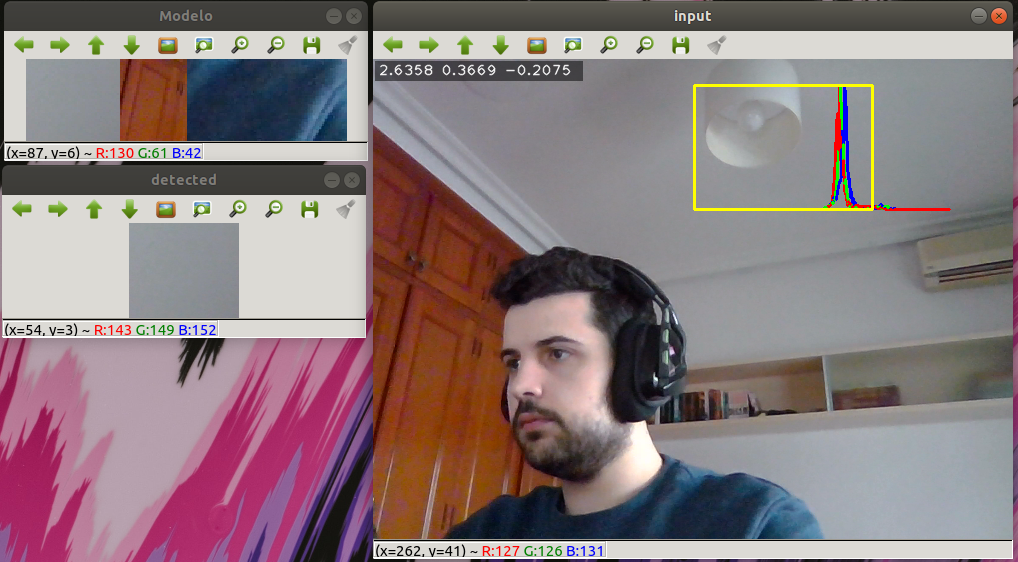
\includegraphics[width=10cm]{imagenes/histo.png}
	\caption{Comparación de histogramas}
	\label{fig:hist}
\end{figure}

El archivo que contiene el programa de \textit{Segmentación de color} tiene el nombre de \textit{segcolor.py}.

\begin{tcolorbox}[collower=red!75!black]
	python \textbf{segcolor.py}
	\tcblower
	- -dev : Seleccionar dispositivo de entrada.
\end{tcolorbox}

Operaciones durante la ejecución:

\begin{center}
	\begin{tabular}{ l | c }
		Tecla & Acción \\ \hline
		c & Guardar zona ROI \\
		x & Eliminar zona ROI \\
		m & Almacenar histogramas del ROI en el modelo \\
	\end{tabular}
\end{center}

\newpage

%------------------------------------------------

\section{FILTROS}
\bigskip

\begin{tcolorbox}[breakable,notitle,boxrule=0pt,colback=lightgray,colframe=lightgray]
Muestra el efecto de diferentes filtros sobre sobre la imagen en vivo de la webcam. Selecciona con el teclado el filtro deseado y modifica sus posibles parámetros (p.ej. el nivel de suavizado) con las teclas o con trackbars. Aplica el filtro en un ROI para comparar el resultado con el resto de la imagen. Opcional: implementa en Python o C "desde cero" algún filtro y compara la eficiencia con OpenCV.
\end{tcolorbox}

Para la realización de este ejercicio se ha hecho uso de los siguientes códigos ejemplo proporcionados por el profesor:

\begin{itemize}
  \item roi.py
  \item trackbar.py
\end{itemize}

\textit{OpenCV} dispone de una serie de filtros por defecto, entre estos se implementan \textbf{\textit{boxFilter}} y \textbf{\textit{GaussianBlur}}. El primero se trata de un filtro de suavizado, mientras que el segundo aplica un filtro gausiano.
Asimismo, se implementa un filtro desde cero mediante el uso de la función \textbf{\textit{filter2D}} de openCV y la creación de kernel, que ira recorriendo la imagen aplicando dicho filtro.
\\
\renewcommand{\baselinestretch}{1}
\begin{tcolorbox}[]
\begin{lstlisting}[language=Python]
size = cv.getTrackbarPos("Size", "input")
if size == 0:
    size = 1
            
kernel = np.array([[-1.0, -1.0], 
                   [2.0, 2.0],
                   [-1.0, -1.0]])

kernel = kernel/(np.sum(kernel) if np.sum(kernel)!=0 else 1)
kernel = kernel * size

frame[y1:y2+1, x1:x2+1] = cv.filter2D(frame[y1:y2+1, x1:x2+1], -1, kernel)
\end{lstlisting}
\end{tcolorbox}
\renewcommand{\baselinestretch}{1.5}

Ademas, el programa dispone de un trackbar para poder modificar los tres filtros que estan implementados.

\subsection*{Manual de Usuario}

El archivo que contiene el programa de \textit{Filtros} tiene el nombre de \textit{filtros.py}. Y para ejecutarlo, será necesario introducir el siguiente comando en el directorio donde se encuentre dicho archivo:
\\
\begin{tcolorbox}[collower=red!75!black]
python \textbf{filtros.py}
\tcblower
- -dev : Seleccionar dispositivo de entrada.
\end{tcolorbox}

Operaciones durante la ejecución:

\begin{center}
    \begin{tabular}{ l | c }
      Tecla & Acción \\ \hline
      c & Guardar zona ROI \\
      x & Eliminar zona ROI \\
      b & Mantener para aplicar filtro \textit{boxFilter} \\
      g & Mantener para aplicar filtro \textit{GaussianBlur} \\
      v & Mantener para aplicar filtro \textit{custom} \\
    \end{tabular}
\end{center}

Ejemplo de ejecución del programa:

\begin{figure}[h]
    \begin{subfigure}{0.35\textwidth}
        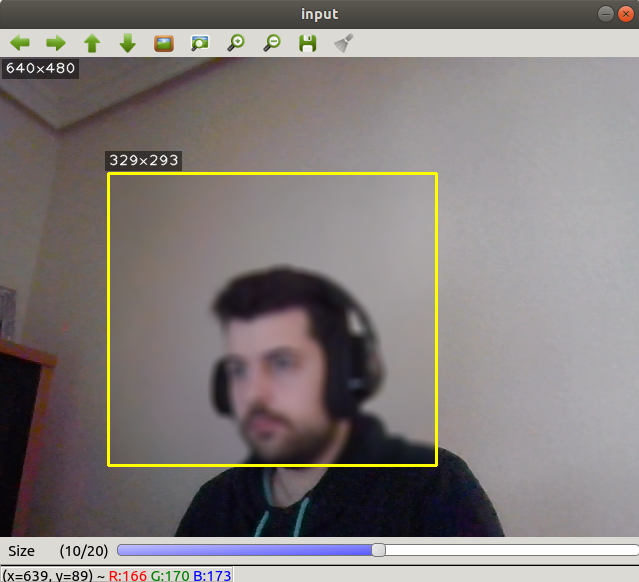
\includegraphics[width=0.9\linewidth, height=5cm]{imagenes/boxFilter.png} 
        \caption{boxFilter}
        \label{fig:boxFilter}
    \end{subfigure}
    \begin{subfigure}{0.35\textwidth}
        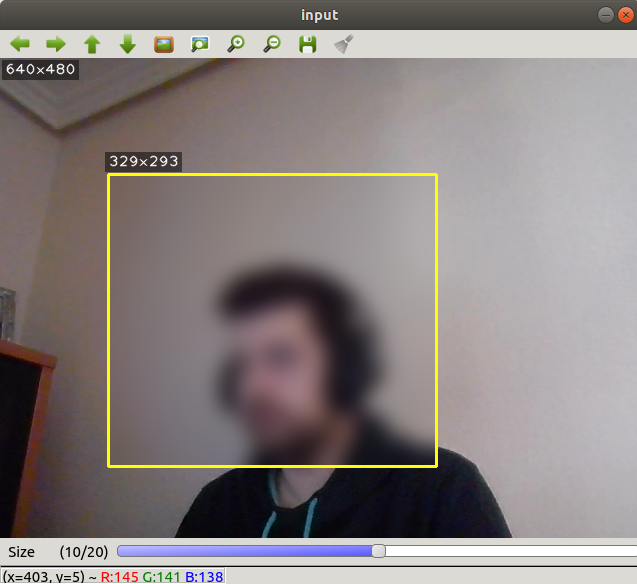
\includegraphics[width=0.9\linewidth, height=5cm]{imagenes/gaussian.png}
        \caption{GaussianBlur}
        \label{fig:Gaussian}
    \end{subfigure}
    \begin{subfigure}{0.35\textwidth}
        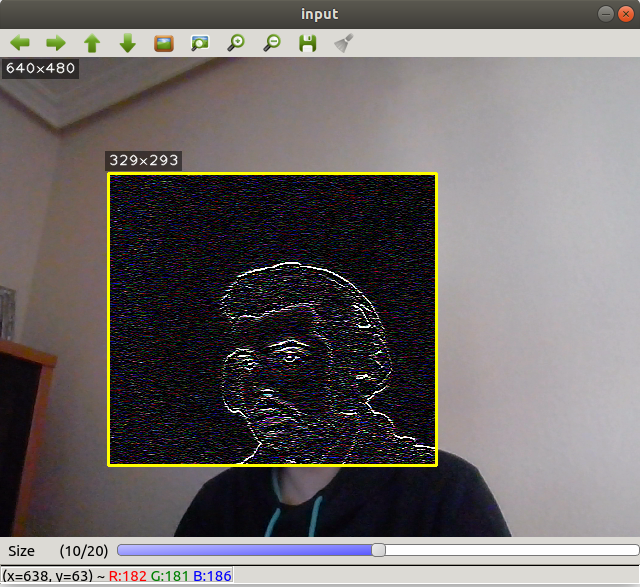
\includegraphics[width=0.9\linewidth, height=5cm]{imagenes/custom.png}
        \caption{CustomFilter}
        \label{fig:custom}
    \end{subfigure}

    \caption{Funcionamiento programa \textbf{filtros.py}}
    \label{fig:filtros}
\end{figure}

\newpage

%------------------------------------------------

\section{SIFT}
\bigskip

\begin{tcolorbox}[breakable,notitle,boxrule=0pt,colback=lightgray,colframe=lightgray]
Escribe una aplicacion de reconocimiento de objetos (p.ej. carátulas de CD, portadas de libros, cuadros de pintores, etc.) con la webcam basada en el número de coincidencias de keypoints.
\end{tcolorbox}

Para la realización de este ejercicio se ha hecho uso de los siguientes códigos ejemplo proporcionados por el profesor:

\begin{itemize}
  \item sift-0.py
  \item sift-1.py
  \item sift.py
\end{itemize}

Este ejercicio trata de encontrar los puntos de interes más importantes de un objeto y crear un modelo con ellos para poder detectarlos en cualquier imagen futura. Para esto, primero habrá que preparar una carpeta con imagenes de los objetos con los que se quiere formar el modelo. En este caso, se creará con imagenes de caratulas de películas, y son las siguientes:
\\

\begin{figure}[htp]
    \centering
    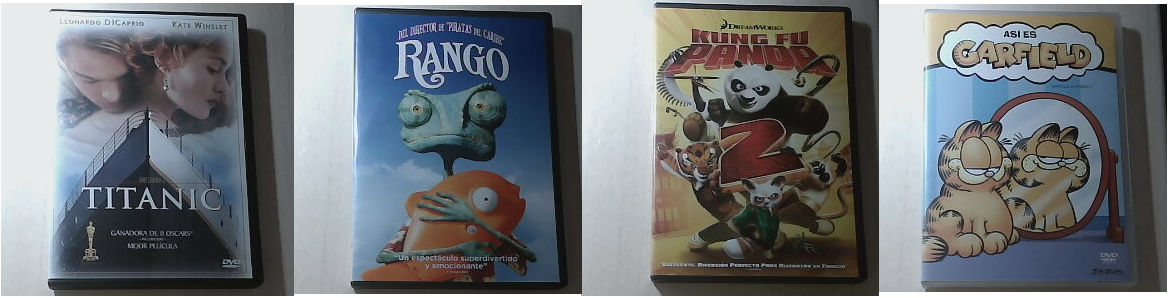
\includegraphics[width=15cm]{imagenes/modelo.png}
    \caption{Imagenes del modelo}
    \label{fig:modelo}
\end{figure}

La obtencion de los puntos de interes de las imagenes del modelo se realiza la función \textbf{\textit{getKeypoints}}. Este realiza uso de una característica de \textit{OpenCV}, llamada SIFT, y se crea con un numero de \textit{features} de 500. Estas serán los puntos de interes totales que se tomarán de una imagen. Asimismo, el programa permite la inclusión de nuevas imagenes en el modelo durante la ejecución de este. El lado malo, es que las imagenes deben estar tomadas en condiciones donde solamente se vea la caratula, sino se crearán puntos que se pueden considerar como \textit{ruido}.
\\
\renewcommand{\baselinestretch}{1}
\begin{tcolorbox}[]
\begin{lstlisting}[language=Python]
def getKeypoints(frame):
    keypoints , descriptors = sift.detectAndCompute(frame, mask=None)
    return keypoints, descriptors
\end{lstlisting}
\end{tcolorbox}
\renewcommand{\baselinestretch}{1.5}

Una vez este cargado el modelo, se podrá hacer la detección de la imagen actual mediante la función \textbf{\textit{bestMatch}} que obtiene el numero de puntos de interes que tiene en común con cada una de la imagen del modelo y devuelve la imagen de este que más coincidencias tiene con la actual.
\\
\renewcommand{\baselinestretch}{1}
\begin{tcolorbox}[]
\begin{lstlisting}[language=Python]
def bestMatch(descriptores, modelo):
    mayorM = 0
    a = 0
    index = 0
    for [d, img] in modelo:
        nMatch = getMatches(descriptores, d)
        #print("Index: ", index, ", Matches: ", nMatch)
        if nMatch > mayorM:
            mayorM = nMatch
            a = index
        index = index + 1
    return a
\end{lstlisting}
\end{tcolorbox}
\renewcommand{\baselinestretch}{1.5}


\subsection*{Manual de Usuario}

El archivo que contiene el programa de \textit{SIFT} tiene el nombre de \textit{sift.py}. Y para ejecutarlo, será necesario introducir el siguiente comando en el directorio donde se encuentre dicho archivo:
\\
\begin{tcolorbox}[collower=red!75!black]
python \textbf{sift.py}
\tcblower
- -dev : Seleccionar dispositivo de entrada.
\end{tcolorbox}

Operaciones durante la ejecución:

\begin{center}
    \begin{tabular}{ l | c }
      Tecla & Acción \\ \hline
      c & Añadir imagen al modelo \\
      m & Cargar modelo, con las imagenes de la carpeta \textit{pelis}\\
      d & Mantener la tecla para realizar la detección \\
    \end{tabular}
\end{center}

Ejemplo de ejecución del programa:

\begin{figure}[htp]
    \centering
    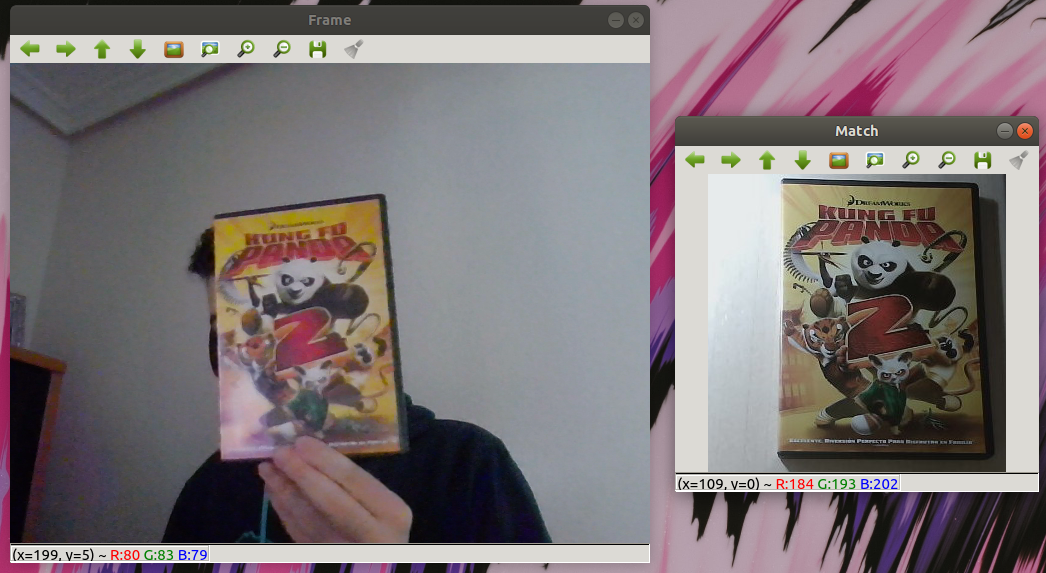
\includegraphics[width=10cm]{imagenes/sift.png}
    \caption{Ejecución de \textit{sift.py}}
    \label{fig:sift}
\end{figure}

\section{RECTIF}
\bigskip

\begin{tcolorbox}[breakable,notitle,boxrule=0pt,colback=lightgray,colframe=lightgray]
	Rectifica la imagen de un plano para medir distancias (tomando manualmente referencias conocidas). Por ejemplo, mide la distancia entre las monedas en coins.png o la distancia a la que se realiza el disparo en gol-eder.png. Verifica los resultados con imágenes originales tomadas por ti.
\end{tcolorbox}

\newpage

%------------------------------------------------

\section{PANO}
\bigskip

\begin{tcolorbox}[breakable,notitle,boxrule=0pt,colback=lightgray,colframe=lightgray]
	Crea automáticamente un mosaico a partir de las imágenes en una carpeta. Las imágenes no tienen por qué estar ordenadas ni formar una cadena lineal y no sabemos el espacio que ocupa el resultado. El usuario debe intervenir lo menos posible. Recuerda que debe tratarse de una escena plana o de una escena cualquiera vista desde el mismo centro de proyección. Debes usar homografías. Compara el resultado con el que obtiene la utilidad de stitching de OpenCV.
\end{tcolorbox}

\newpage

%------------------------------------------------

\section{RA}
\bigskip

\begin{tcolorbox}[breakable,notitle,boxrule=0pt,colback=lightgray,colframe=lightgray]
	Crea un efecto de realidad aumentada interactivo: esto significa que a) los objetos virtuales deben cambiar de forma, posición o tamaño siguiendo alguna lógica; b) el usuario puede observar la escena cambiante desde cualquier punto de vista moviendo la cámara alrededor del marcador; y c) el usuario puede marcar con el ratón en la imagen puntos del plano de la escena para interactuar con los objetos virtuales.
\end{tcolorbox}

\newpage

%------------------------------------------------

\section{DLIB}
\bigskip

\begin{tcolorbox}[breakable,notitle,boxrule=0pt,colback=lightgray,colframe=lightgray]
	Escribe una aplicación de tu invención que utilice los marcadores de cara obtenidos por el shape detector disponible en dlib (ejemplo /hog/facelandmarks.py).
\end{tcolorbox}

\newpage

%------------------------------------------------

\section{VROT}
\bigskip

\begin{tcolorbox}[breakable,notitle,boxrule=0pt,colback=lightgray,colframe=lightgray]
	Estima de forma aproximada la velocidad angular de rotación de la cámara (grados/segundo) analizando las trayectorias obtenidas por el tracker de Lucas-Kanade (ejemplo LK/lk-track.py).
\end{tcolorbox}

\newpage

%------------------------------------------------

\section{DELOGO}
\bigskip

\begin{tcolorbox}[breakable,notitle,boxrule=0pt,colback=lightgray,colframe=lightgray]
	Detecta el logotipo de una cadena de TV en una emisión por streaming y suprime los cortes publicitarios.
\end{tcolorbox}

\newpage

%------------------------------------------------

\section{SILU}
\bigskip

\begin{tcolorbox}[breakable,notitle,boxrule=0pt,colback=lightgray,colframe=lightgray]
	Escribe una aplicación de reconocimiento de siluetas con la webcam basado en descriptores frecuenciales.
\end{tcolorbox}

\newpage

%------------------------------------------------

\section{ANON}
\bigskip

\begin{tcolorbox}[breakable,notitle,boxrule=0pt,colback=lightgray,colframe=lightgray]
	Modifica el ejemplo de reconocimiento de caras DL/facerec para seleccionar caras pinchando con el ratón (o tomándolas de un directorio) para que cuando se reconozcan en las imágenes se oculten (emborronándolas o pixelizándolas).
\end{tcolorbox}

\newpage

%------------------------------------------------

\section{CR}
\bigskip

\begin{tcolorbox}[breakable,notitle,boxrule=0pt,colback=lightgray,colframe=lightgray]
	Reproduce la demostración del cross-ratio de 4 puntos en una recta del tema de transformaciones del plano. Marca tres puntos con el ratón y añade automáticamente tres más y el punto de fuga, suponiendo que en el mundo real los puntos están alineados y a la misma distancia.
\end{tcolorbox}

\newpage

%------------------------------------------------

\section{SWAP}
\bigskip

\begin{tcolorbox}[breakable,notitle,boxrule=0pt,colback=lightgray,colframe=lightgray]
	Intercambia dos cuadriláteros en una escena marcando manualmente los puntos de referencia.
\end{tcolorbox}

\newpage

%------------------------------------------------

\section{NFACE}
\bigskip

\begin{tcolorbox}[breakable,notitle,boxrule=0pt,colback=lightgray,colframe=lightgray]
	Implementa la normalización de caras explicada en la sección de transformaciones afines.
\end{tcolorbox}

\newpage

%------------------------------------------------

\section{DNI}
\bigskip

\begin{tcolorbox}[breakable,notitle,boxrule=0pt,colback=lightgray,colframe=lightgray]
	Sustituye la foto de un carnet que se observa en una imagen en vivo.
\end{tcolorbox}

\newpage

%------------------------------------------------

\section{SUDO}
\bigskip

\begin{tcolorbox}[breakable,notitle,boxrule=0pt,colback=lightgray,colframe=lightgray]
	Haz un programa capaz de rellenar un sudoku que se observa en una imagen en vivo.
\end{tcolorbox}

\newpage

%------------------------------------------------

\section{STC}
\bigskip

\begin{tcolorbox}[breakable,notitle,boxrule=0pt,colback=lightgray,colframe=lightgray]
	Resuelve los problemas planteados en el notebook stereo-challenge.
\end{tcolorbox}

\newpage

%------------------------------------------------

\section{PROBLEMA ORIGINAL}
\bigskip

\begin{tcolorbox}[breakable,notitle,boxrule=0pt,colback=lightgray,colframe=lightgray]
	Problema Original.
\end{tcolorbox}

\newpage

%----------------------------------------------------------------------------------------
%	REFERENCE LIST
%----------------------------------------------------------------------------------------

\bibliographystyle{plain}
\bibliography{ecl.bib}

%----------------------------------------------------------------------------------------

\end{document}
